\section{Qu'est-ce qu'un labyrinthe ?}
\subsection{Définition d'un labyrinthe}
Un labyrinthe est une structure complexe de passages reliés entre-eux. L’objectif du solveur est de passer d'un point de départ à un point d'arrivée, c'est-à-dire trouver le passage reliant ces deux points. Le labyrinthe est une énigme qui teste l'intelligence, la réflexion, et la rapidité d'exécutions du solveur. D'un point de vu mathématique, les labyrinthes peuvent êtres représentés comme étant des surfaces connexes. 


\subsection{Histoire et application}
Le mot labyrinthe trouve son origine dans la  mythologie grecque, c'était une structure constitué de galeries, construite par Dédale afin d'y enfermer le Minotaure.
Le divertissement et l'entraînement cérébral peuvent être considérés comme les principaux objectifs d'application d'un labyrinthe.
En ce qui concerne le domaine scientifique, les labyrinthes peuvent être vu comme des supports pour effectuer des démonstrations robotiques. Le concept de labyrinthe a permis la naissance de concours robotiques comme les compétitions Micromouses ou l'objectif est de résoudre une énigme (un labyrinthe) en ayant recours à différents algorithmes d'intelligence artificielle.
\section{Classification d'un labyrinthe} 
\label{sec:ProblematiqueConstructionLabyrinthe}
\paragraph{}
Les labyrinthes (et les algorithmes responsables de leur génération) peuvent être organisés selon trois critères de  classifications différents. Ces critères sont : la dimension, la topologie, et la tessellation. Un labyrinthe peut prendre un objet d'un de ses classes dans n'importe quelle combinaison.

\subsection{Dimension d'un labyrinthe}
La dimension d'un labyrinthe corresponds à l'espace dimensionnel couvert par le labyrinthe. Les labyrinthes peuvent êtres de dimensionnalité 2, 3 ou tout autre dimension supérieure.

\begin{figure*}[htp] 
    \centering
    \subfloat[Labyrinthe en 2 dimensions.]{%
        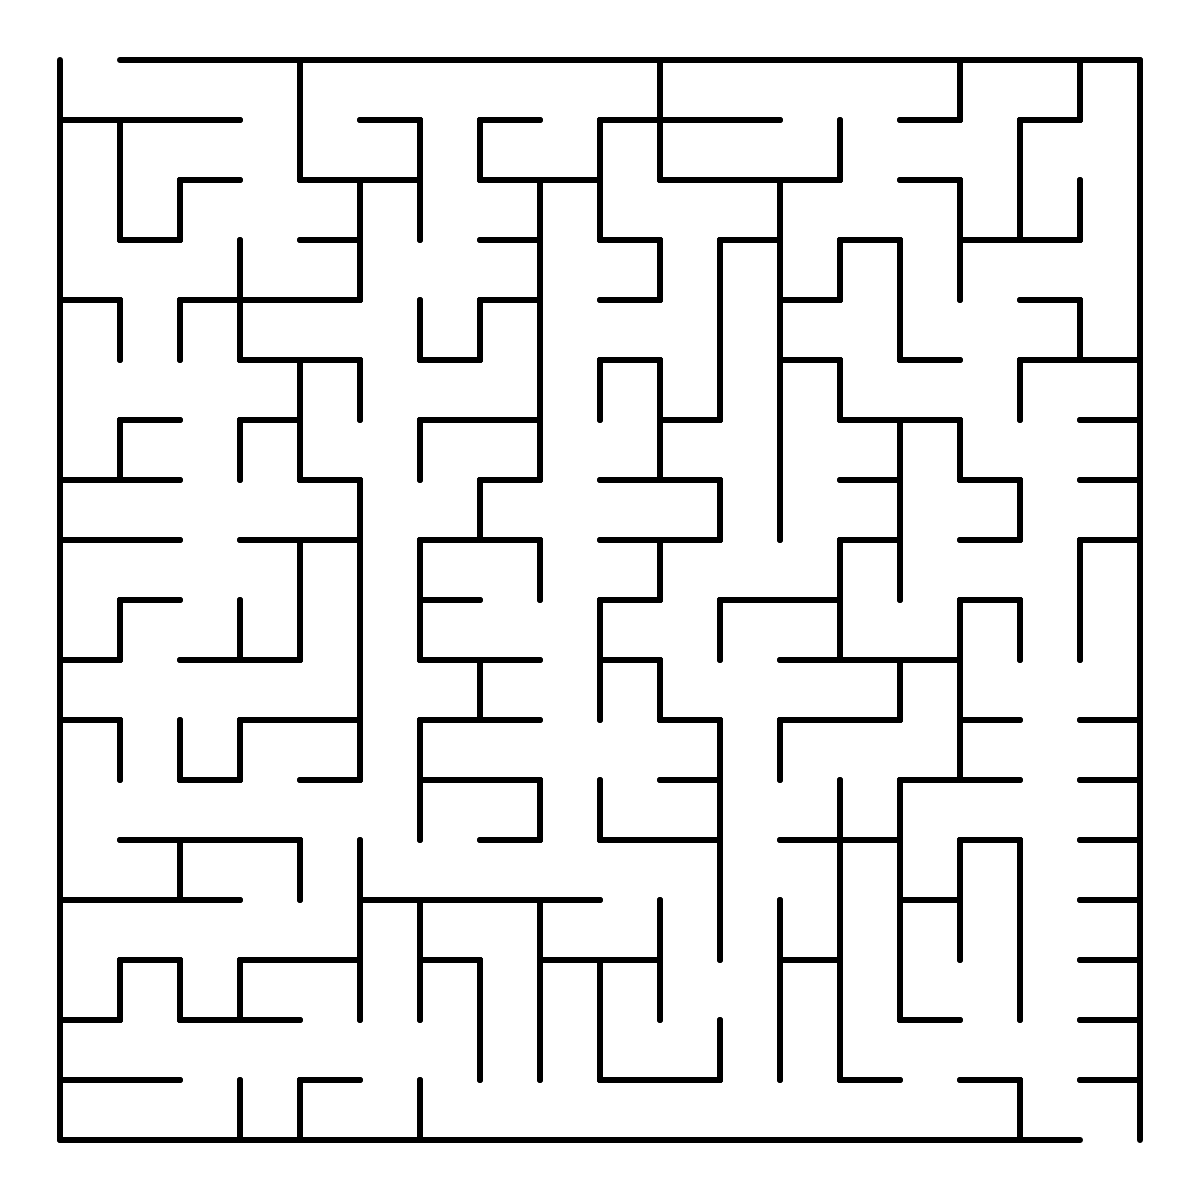
\includegraphics[width=0.35\textwidth]{report/pics/2D_maze.png}%
        \label{fig:a}%
        }%
    \hfill%
    \subfloat[Labyrinthe en 3 dimensions.]{%
        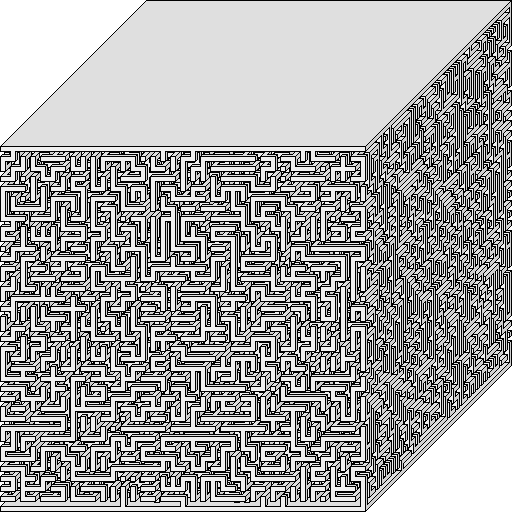
\includegraphics[width=0.35\textwidth]{pics/3D_maze.png}%
        \label{fig:b}%
        }%
    \caption{Exemple d'un labyrinthe 2D et d'un labyrinthe 3D}
\end{figure*}


\subsection{Tessellation d'un labyrinthe}
La classe de tessellation est la géométrie des cellules individuelles qui composent le labyrinthe. Il existe de nombreux types de tessellation, on citera notamment :
\begin{itemize}
\item\textbf{ Tesellation orthogonale :} Il s'agit d'une grille rectangulaire standard où les cellules ont des passages qui se coupent à angle droit formant des cellules sous forme de carrés.

\item\textbf{Tesellation delta :} Un labyrinthe à tessellation delta est un composé de triangles imbriqués, où chaque cellule peut avoir jusqu'à trois passages connectés.

\item\textbf{Tesellation theta :} Un labyrinthe à tessellation theta est composé de cercles concentriques. Les cellules ont généralement quatre connexions de passage possibles, mais peuvent en avoir plus en raison du plus grand nombre de cellules dans les anneaux externes.
\end{itemize}

\begin{figure*}[htp] 
    \centering
    \subfloat[Labyrinthe orthogonal.]{%
        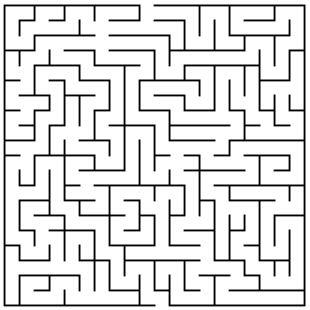
\includegraphics[width=0.27\textwidth]{report/pics/orthogonal_maze.png}%
        \label{fig:a}%
        }%
    \hfill%
    \subfloat[Labyrinthe delta.]{%
        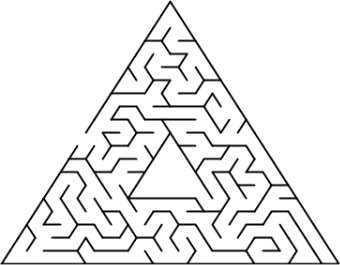
\includegraphics[width=0.3\textwidth]{report/pics/delta_maze.png}%
        \label{fig:b}%
        }%
        \hfill%
    \subfloat[Labyrinthe theta.]{%
        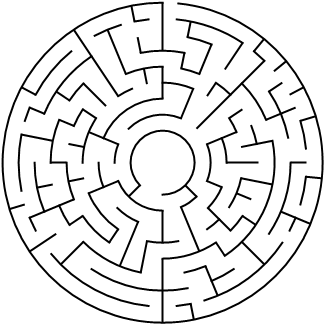
\includegraphics[width=0.3\textwidth]{report/pics/theta_maze.png}%
        \label{fig:c}%
        }%
    \caption{Exemple de labyrinthes avec différentes classes de tessellation.}
\end{figure*}


\subsection{Topologie d'un labyrinthe}
D’un point de vu mathématique, un labyrinthe est définie comme étant une surface connexe pouvant avoir deux types de topologies : topologie simple et topologie comportant des anneaux. Cette différence dans le type de topologie conduit à une distinction des labyrinthes en deux catégories : Les labyrinthes parfaits et les labyrinthes imparfaits.

\subsubsection{Labyrinthe parfait}
Afin qu'un labyrinthe soit labélisé comme étant parfait, ce dernier doit remplir deux conditions :
\begin{itemize}
\item Ne contient pas de cycles.
\item Il existe un unique chemin entre la cellule de départ et la cellule d’arrivée du labyrinthe.
\end{itemize}
Plus généralement, quelque soit deux cellules sélectionnées dans notre labyrinthe, le chemin entre ces deux cellules doit être unique.

\subsubsection{Labyrinthe imparfait}
Un labyrinthe qui ne remplit pas les conditions pour être labélisé comme parfait est dit imparfait. Les labyrinthes imparfaits peuvent donc contenir des boucles, des îlots ou des cellules inaccessibles.


\begin{figure*}[htp] 
    \centering
    \subfloat[Labyrinthe parfait.]{%
        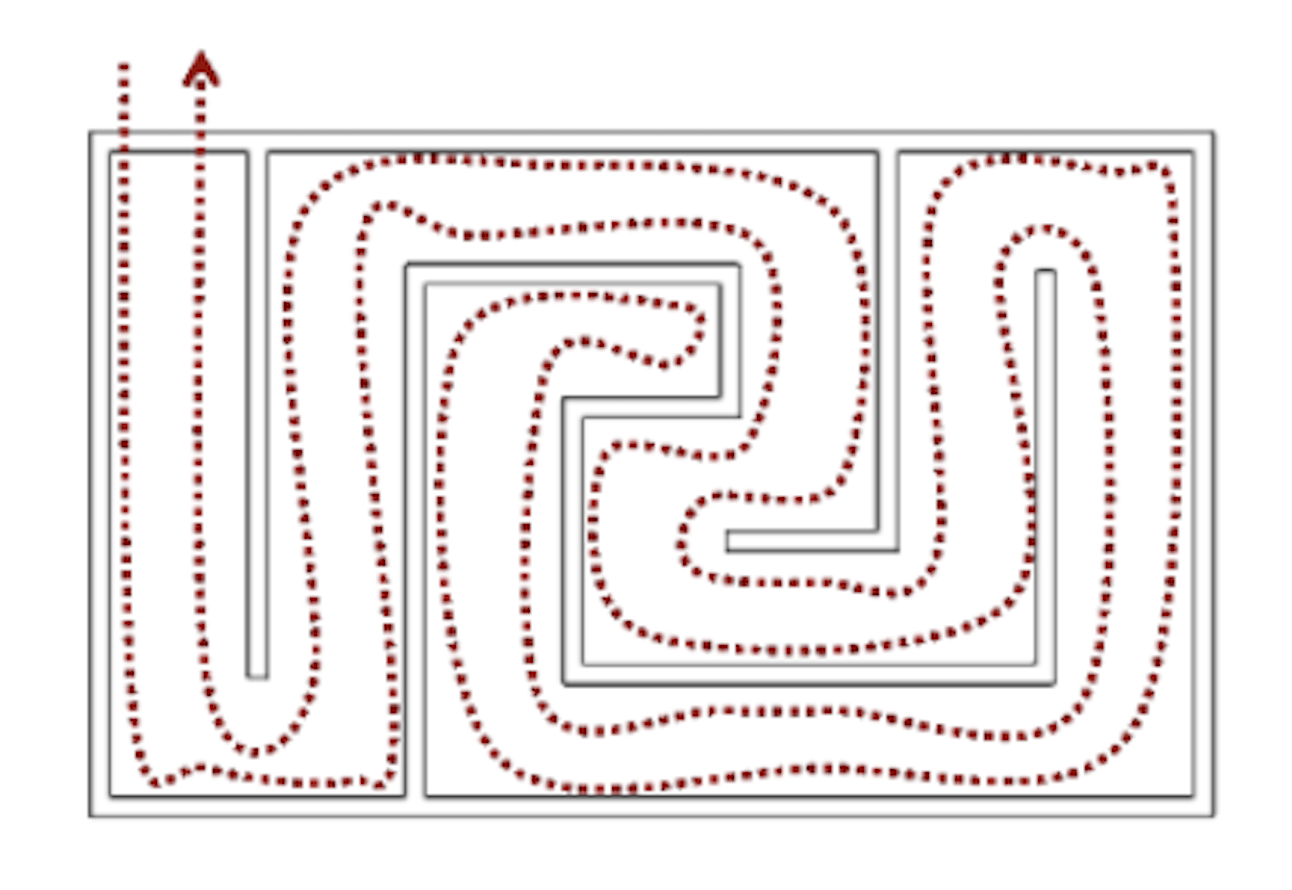
\includegraphics[width=0.5\textwidth]{report/pics/perfect_maze.png}%
        \label{fig:a}%
        }%
    \hfill%
    \subfloat[Labyrinthe imparfait.]{%
        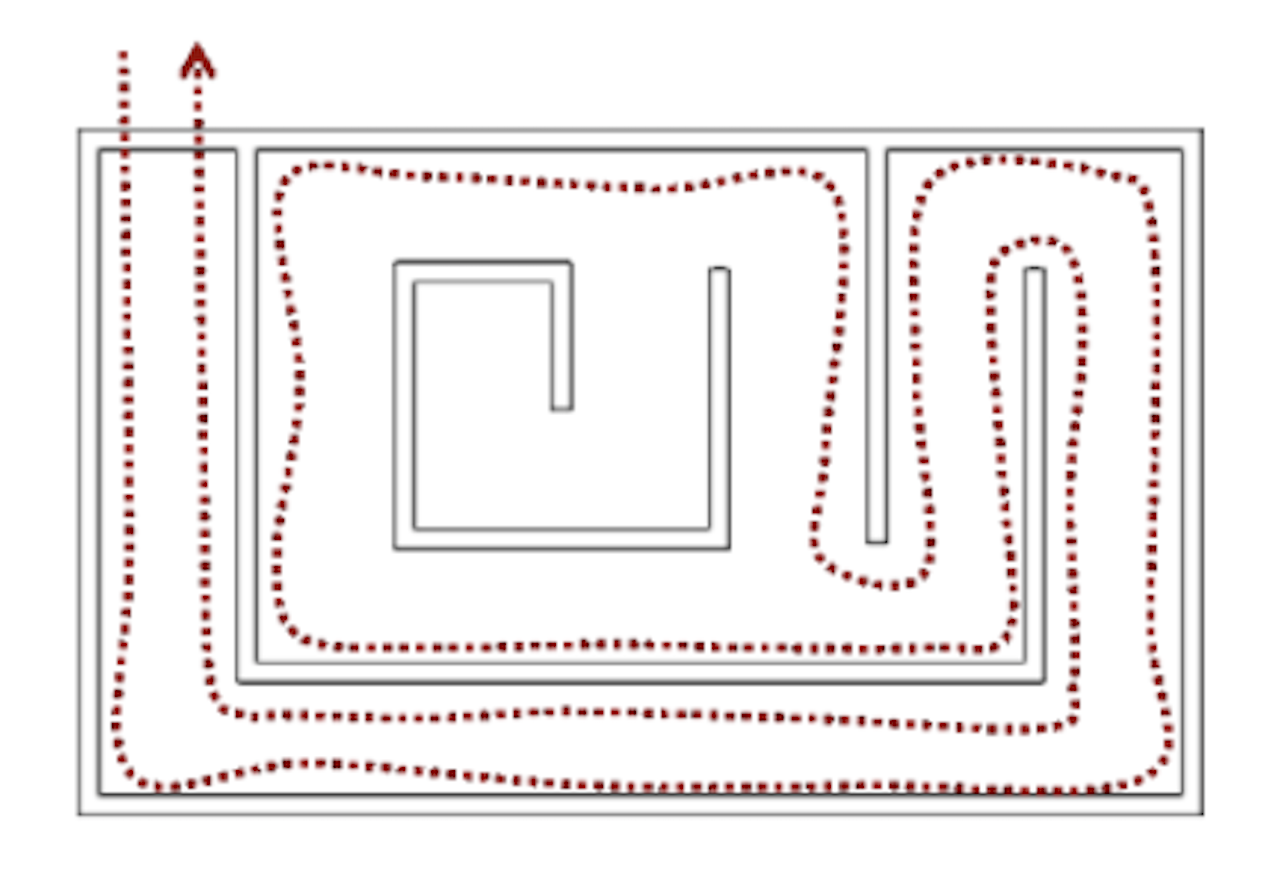
\includegraphics[width=0.5\textwidth]{report/pics/imperfect_maze.png}%
        \label{fig:b}%
        }%
    \caption{Exemple d'un labyrinthe parfait et d'un labyrinthe imparfait.}
\end{figure*}




Dans la suite de ce rapport, nous considérons l'ensemble de nos labyrinthes comme étant de dimension 2 et possédant une tessellation orthogonale. La distinction se feras sur le critère de la topologie, on distinguera alors deux types de labyrinthes : les labyrinthes parfaits et les labyrinthes imparfaits.

\newpage
\section{Introduction à la génération de labyrinthes}
Les algorithmes utilisés pour la génération de labyrinthes suivent un ordre d'étapes prédéfini. Afin de créer des labyrinthes structurés de manière aléatoire, une ou plusieurs étapes de l'algorithme doivent être randomisées (c'est-à-dire que la prise de décision au sein de l'étape doit utiliser une fonction renvoyant un résultat aléatoire). 
Il existe deux approches algorithmiques générales utilisées pour la génération automatisée des labyrinthes. Ces approches sont : l'ajout de murs et la sculpture de passages.
\\
\begin{itemize}
\item\textbf{ Ajout de murs :} Dans cette approche, on se base sur l'ajout de murs pour générer progressivement notre labyrinthe. On démarre d'un labyrinthe vide, puis l'algorithme va placer au fur et à mesure des murs à des positions spécifiques. 
\\
\item\textbf{ Sculpture de passages :} Les algorithmes basés sur cette approche se concentrent sur les chemins et le positionnement des cellules du labyrinthe. On démarre d'une matrice de cellules (une grille complètement remplie de murs), puis l'algorithme de sculpture de passages va alors creuser à travers la grille et détruire certains murs reliant les différentes cellules, ce processus itérative générera au final un labyrinthe.
\end{itemize}



\subsection{Rappels sur la théorie des graphes}
Cette sous-section présente certains principes fondamentaux de la théorie des graphes sur lesquels sont basé les algorithmes de génération de labyrinthes. 
\subsubsection{Graphe}
Un graphe est le concept fondamental dans la théorie des graphes, ce dernier est définie comme étant un triplet  $G = (V, E, \epsilon )$, avec $V$ représentant l'ensemble des sommets, $E$  l'ensemble des arêtes et $\epsilon$ une fonction de mappage appelée relation d'incidence tel que $\epsilon : E	\rightarrow V^2$

\subsubsection{Arbre}
Un arbre est un graphe connexe non orienté ne contenant pas de cycles, c'est-à-dire qu'il existe exactement un seul et unique chemin entre chaque paire de sommets du graphe. Un graphe connexe avec $n$ sommets et $n-1$ arêtes est un arbre.
La suppression de toute les arête entraînerait la perte de connexité du graphe, et l'ajout d'une arête créerait un cycle au sein du graphe.

\subsubsection{Arbre couvrant}
Soit $G$ un graphe. L'arbre couvrant de $G$ est le sous graphe qui est connexe, sans cycle et contient tous les sommets de $G$.


\newpage
\subsection{Théorie des graphes et labyrinthes.}
Sur la figure ci-dessous on peut apercevoir deux labyrinthes. Celui de gauche est un labyrinthe parfait, celui de droite un labyrinthe imparfait (car il contient des boucles). Il existe une autre approche pour visualiser nos labyrinthes. Au lieu de penser aux murs constituants le labyrinthe, nous pouvons penser aux chemins entre les cellules. 
Les chemins à l'intérieur du labyrinthe forment un graphe. Le graphe de chaque labyrinthe est illustré ci-dessous en rouge. \newline
\fig{pics/graphe_theory.png}{12cm}{9cm}
{Géénration d'un labyritnhe 3*3 à l'aide de l'algortihme d'arbre binaire.}{mmcomp}


Dans le cas du labyrinthe imparfait à droite, on va bien qu'il existe une boucle à l'intérieur du graphe.
\fig{pics/graph_theory3.png}{10cm}{7cm}
{Modélisation des labyritnhes sous forme de graphes.}{mmcomp}

De cela, nous arrivons à la conclusion que la génération d'un labyrinthe parfait aléatoire consiste à générer un arbre couvrant aléatoire qui relie toutes les cellules du labyrinthe.
Les différentes procédures et approches utilisées pour la génération d'arbres couvrant forment les bases des différents algorithmes de génération de labyrinthes. 


\section{État de l’art: études des solutions existantes} \label{sec:etatDeLart2}
Dans cette section, nous passons en revue certains des algorithmes les plus populaires utilisés pour la génération de labyrinthes parfaits.
L'ensemble des algorithmes présentés dans cette section suivent l'approche "sculpture de passages" pour générer un labyrinthe. Pour chaque algorithme, on démarre à chaque fois d'une grille remplie de murs, puis l'algorithme se chargera de creuser un chemin parmis ces murs afin de construire son labyrinthe. 
\subsection{Algorithme de Kruskal}
Le générateur de labyrinthe Kruskal est une version aléatoire de l'algorithme de Kruskal. C'est un algorithme qui permet de produire un arbre couvrant pour un graphe (un labyrinthe parfait).
L'algorithme de Kruskal randomnisé pour la génération de labyrinthe fonctionne de la manière suivante :
\newline
\begin{enumerate}
    \item On démarre d'un labyrinthe sous de grille complètement remplie de murs. On regroupe tous les murs séparant les cellules du labyrinthe dans un ensemble.
    \item On choisit un mur à partir de cet ensemble de manière aléatoire et on le supprime du labyrinthe.
    \item On réitère l'opération jusqu'à ce qu'il n'y est plus aucune cellule isolée.
\end{enumerate}
\fig{pics/kruskal.png}{16cm}{12cm}
{Géénration d'un labyritnhe 3*3 à l'aide de l'algortihme de Kruskal.}{mmcomp}


\subsection{Algorithme d'arbre binaire}
L'algorithme de génération de labyrinthes "Arbre Binaire" est l'un des algorithmes les plus simples utilisé pour la génération de labyrinthe parfaits. Une des spécificités de l'algorithme est qu'il n'a pas besoin de sauvegarder en mémoire l'état des cellules du labyrinthe. Il peut construire un labyrinthe entier en regardant une seule cellule à la fois.
Son principe de fonctionnement est très simple :
\newpage
\begin{enumerate}
    \item Pour chaque cellule au sein du labyrinthe, exécuter les étapes deux et trois.
    \item Si ils existent, récupérer les voisins se situant au nord et à l'ouest de la cellule.
    \item On choisit un mur à partir de cet ensemble de manière aléatoire et on le supprime du labyrinthe.
    \item Sélectionner un des voisins de manière aléatoire, et perforer le mur reliant la cellule et le voisin choisit.
\end{enumerate}
\newline
\fig{pics/binary_tree.png}{10cm}{7cm}
{Géénration d'un labyritnhe 3*3 à l'aide de l'algortihme d'arbre binaire.}{mmcomp}



\subsection{Algorithme de Prim}
Dans l'algorithme de Kruskal, on effectuait une sélection aléatoire parmis les murs du labyrinthe qu'on supprimait. L'algorithme de Prim aborde le problème de génération de labyrinthe sous un angle différent, ici, on démarre à partir de n'importe quelle cellule puis à partir de cette cellule l'algorithme va se charger de développer un chemin jusqu'à ce qu'on obtienne un labyrinthe parfait.
L'algorithme de Prim randomnisé pour la génération de labyrinthe suit les étapes suivantes :

\begin{enumerate}
    \item On choisit une cellule de départ de manière aléatoire qu'on ajoute à l'ensemble V.
    \item On choisit une cellule aléatoire C de l'ensemble V dont au moins un des voisins n'appartient pas encore à l'ensemble V. 
    \item On choisit un voisin aléatoir de la cellule C et on perfore le mur reliant ces deux cellules. On ajoute le voisin choisit à l'ensemble V. 
    \item On réitère les étapes deux et trois jusqu'à ce que l'ensemble V contienne toutes les cellules du labyrinthe.
\end{enumerate}
\newpage
Sur la figure ci-dessous on est illustrée la génération d'un labyrinthe à l'aide de l'algorithme de Prim étape par étape. Les cellules appartenant à l'ensemble V (au labyrinthe) sont marquées en blanc, leurs cellules voisines en rose et en jaune on marque à chaque quelle cellule a été chosiit de manière aléatoire.
\fig{pics/prim.png}{16cm}{12cm}
{Géénration d'un labyritnhe 3*3 à l'aide de l'algortihme de Prim.}{mmcomp}

\subsection{Algorithme de Backtracking}
Le Backtracking est une approche et une famille d'algorithmes utilisés pour résoudre des problèmes algorithmiques.
Un algorithme de Backtracking (en français retour en arrière) est un algorithme récursif qui tente de résoudre un problème donné en testant tous les chemins possibles vers une solution jusqu'à ce qu'une solution soit trouvée. 
Chaque fois qu'un chemin est testé, si aucune solution n'est trouvée, l'algorithme revient en arrière pour tester un autre chemin possible. L'algorithme réitère cette logique jusqu'à ce qu'une solution soit trouvée ou que tous les chemins aient été Le Backtracking est donc un parcours en profondeur sur l'arbre de décision du problème, avec possibilité de revenir en arrière. En ce qui concerne l'algorithme de Backtracking pour la génération de labyrinthe parfait, on verra dans la section suivante que ça sera l'algorithme choisit pour générer les labyrinthes dans lequels va évoluer la Micromouse. On reviendra en détails sur cet algorithme et sa logique de fonctionnement dans la section \textbf{3.6.1.}

\newpage
\section{Comparaison des algorithmes de génération de labyrinthes}
\subsection{Introduction à la comparaison de labyrinthes}
Maintenant qu'on a présenté un ensemble d'algorithmes utilisés pour la génération de labyrinthes parfaits, il faut se décider sur l'algorithme à implémenter afin de générer les labyrinthes dans lequels va évoluer notre Micromouse. Dans cette section, nous présentons les critères et métriques sur lequels on s'est basé afin de comparer les différents algorithmes ainsi que les labyrinthes qu'ils génèrent. Cette section se basent en grande partie sur les recherches et analyses menées et présentées dans le livre "Maze pour Programmers"\cite{maze_for_programmers}.
\newline
Dans ce livre, les différents algorithmes de génération de labyrinthes sont comparés à l'aide des statistiques. Chaque algorithme est exécuté un nombre précis de fois pour générer des labyrinthes de taille fixe. Il suffit alors de choisir une propriété précise et d'analyser les labyrinthes résultants.
\subsection{Critères de comparaison de labyrinthes}


\subsubsection{Impasse}
Une impasse est définie comme une cellule qui n'est liée qu'à un seul voisin, c'est à dire une cellule qui ne possède qu'un seul mur perforé, ces autres murs étant fermés.
Un labyrinthe avec peu d'impasses aura tendance à contenir plus de routes secondaires, ce qui aura pour effet de rendre le labyrinthe plus difficile à résoudre. 
\newline
D'un point de vu de la Micromouse, et dans le but de tester l'intelligence de cette dernière, on préférera un labyrinthe contenant peu d'impasses afin de pouvoir mettre à épreuve les capacités de décisions de cette dernière. Par exemple, dans un labyrinthe contenant un nombre important d'impasses, on pourrait programmer la Micromouse de sorte qu'elle se contente d'avancer sans réel objectif et qu'elle revienne sur ses pas dans la cas ou elle tombe sur impasse et sauvegarde en mémoire la position de cette dernière. 
Ce n'est clairement pas intéressant comme algorithme de navigation, ce qui nous conforte dans notre choix d'opter pour un algorithme qui génère peu d'impasses. La figure suivante montre le nombre moyen d'impasses générées au sein du labyrinthe par différents algorithmes.

\fig{pics/impasse.png}{14.5cm}{12cm}
{Moyenne d'impasses engendrées par différents algorithmes de génération de labyrinthes}{mmcomp}


On constate que l'algorithme de Prim a tendance à produire des labyrinthes où environ 45\% des cellules sont des impasses. En parallèle l'algorithme de Backtracking en génère un nombre beaucoup moins important.


\subsubsection{Variation de directions}
La variation de directions est une mesure de la fréquence à laquelle un passage change de direction. Il est pris comme le pourcentage de cellules avec un passage entrant sur un côté et sortant à gauche ou à droite.
Dans un labyrinthe un faible variation de directions, la majorité des chemins seront des passages droits (horizontaux ou verticaux). Toujours dans l'optique d'utilisation du labyrinthe comme environnement pour la Micromouse, un labyrinthe à faible taux de variation n'est pas intéressant, en effet, l'intelligence de le Micromouse sera mise à l'épreuve lorsque cette dernière devra faire des décisions, l'objectif étant de choisir la direction assurant une solution optimale. Dans le cas de passages en ligne droite, la Micromouse ne fera qu'avancer tout droit en attendant de tomber sur un virage.


\fig{pics/variation_directions}{16cm}{12cm}
{Taux de variation de directions moyens pour différents algorithmes de génération de labyrinthes}{mmcomp}
On s'aperçoit que l'algorithme de Backtracking dispose d'un fréquence de variation de directions de quasiment 50\%, tandis que l'algorithme de Kruskal, de Prim et d'arbre binaire ont des fréquences de variations plus petites.
\subsection{Conclusion}

\newpage


\section{Solution proposée et sa mise en œuvre} \label{sec:solution2}
\subsection{Algorithme de Backtracking pour la génération de labyrinthes parfaits}
Les bases de l'algorithme Backtracking pour la génération de labyrinthes parfaits est qu'on démarre à partir d'une cellule prise au hasard de notre labyrinthe, et qu'on "creuse" un chemin dans une direction aléatoire (haut, bas, gauche, droite). La contrainte est qu'on ne peut jamais creuser vers une cellule qu'on a déjà visitée. À chaque itération, l'algorithme garde en mémoire les cellules visitées et les voisins des ces dernières. Dans le cas ou on arrive sur une cellules dont l'ensemble des voisins ont déjà été visités, on revient en arrière jusqu'à ce qu'on trouve une cellule à qui il reste des voisins non visités. On utilisera une pile comme structure de données afin de stocker les cellules visitées. Le pseudo code de l'algorithme est le suivant : 
\newline
\begin{enumerate}
    \item Choisir une cellule de départ aléatoire, la marquer comme visitée et l'empiler.
    \item Tant que la pile n'est pas vide :
    \begin{enumerate}
        \item Dépiler une cellule de la pile et la marquer comme visitée.
        \item Si la cellule actuelle possède des voisins qui n'ont pas encore été visités :
        \begin{enumerate}
            \item Choisir au hasard un des voisins non visité. \item Supprimer le mur reliant la cellule actuelle et le voisin choisi.
            \item Empiler la cellule actuelle dans la pile et se déplacer vers le voisin choisi.
            \newline
        \end{enumerate}
    \end{enumerate}
\end{enumerate}

Pour une meilleure compréhension, nous allons illustrer et expliciter la génération d'un labyrinthe par l'algorithme de Backtracking étape par étape. Nous utiliserons une pile afin de garder une trace des cellules que nous avons visitées.
On rappelle qu'un pile ne peut être manipulé que via ses opération "empiler" et "dépiler", ce qui assure un ordre précis avec lequel ses éléments sont consultés, ordre tout à fait adapté à l'algorithme de Backtracking dans lequel on souhaite ajouter des cellules au fur et à mesure de leur découverte et les dépiler dès qu'elles ne possèdent plus de voisins nos visités.

\begin{minipage}{0.6\textwidth}
Au départ de l'algorithme, on choisit une cellule aléatoire du labyrinthe qu'on empile dans notre pile. Dans notre exemple on démarre avec la cellule A4. À chaque itération, la cellule au sommet de la pile est considérée comme étant la cellule actuelle.
\end{minipage}
\begin{minipage}{0.4\textwidth}
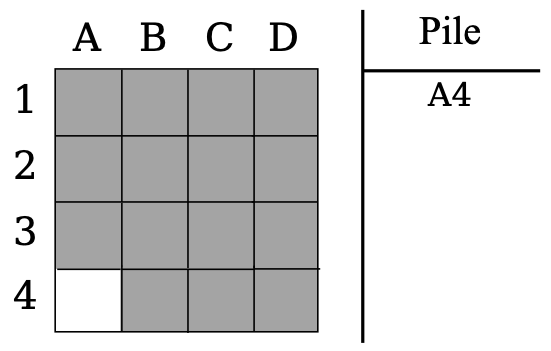
\includegraphics[width=\linewidth]{report/pics/backtracking1.png}
\end{minipage}

\begin{minipage}{0.6\textwidth}
On choisit un voisin aléatoire de la cellule actuelle (dans notre exemple A3) et on supprime le mur qui sépare les deux cellules. On empile le voisin choisit dans notre pile, ce qui en fait la nouvelle cellule actuelle.
\end{minipage}
\begin{minipage}{0.4\textwidth}
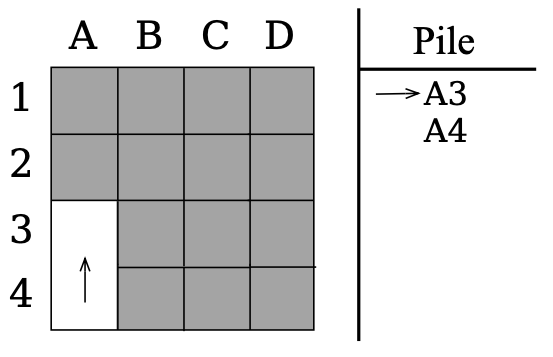
\includegraphics[width=\linewidth]{report/pics/backtracking2.png}
\end{minipage}

\newpage

\begin{minipage}{0.6\textwidth}
Ce processus itérative se poursuit, on explore aléatoirement les cellules voisines comme on peut le voir sur la figure. Chaque cellule visitée sera ajouter à notre pile.
\end{minipage}
\begin{minipage}{0.4\textwidth}
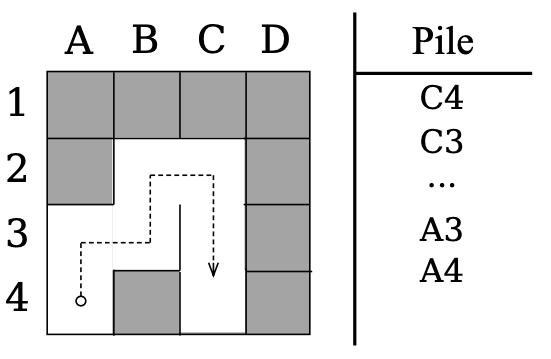
\includegraphics[width=\linewidth]{report/pics/backtracking3.png}
\end{minipage}



\begin{minipage}{0.6\textwidth}
Notre processus aléatoire nous emmène vers la cellule B4 qui elle ne dispose pas de voisins nos visités.
\end{minipage}
\begin{minipage}{0.4\textwidth}
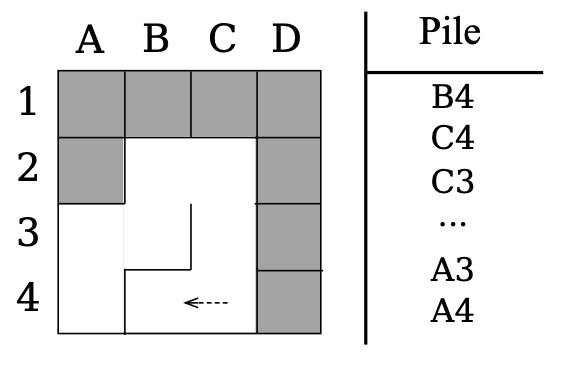
\includegraphics[width=\linewidth]{report/pics/backtracking4.png}
\end{minipage}


\begin{minipage}{0.6\textwidth}
À cette étape, on dépile la cellule B4 de notre pile car elle ne possède plus de voisins non visités. Cette opération a pour effet de faire de la cellule précédente (cellule C4) la nouvelle cellule actuelle de l'algorithme.
\end{minipage}
\begin{minipage}{0.4\textwidth}
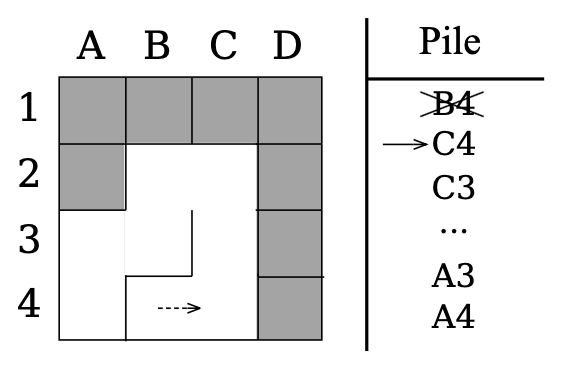
\includegraphics[width=\linewidth]{report/pics/backtracking5.png}
\end{minipage}

\begin{minipage}{0.6\textwidth}
La cellule C4 dispose encore d'un voisin non visité (D4). On poursuit alors notre exploration aléatoire en choisissant ce voisin.
\end{minipage}
\begin{minipage}{0.4\textwidth}
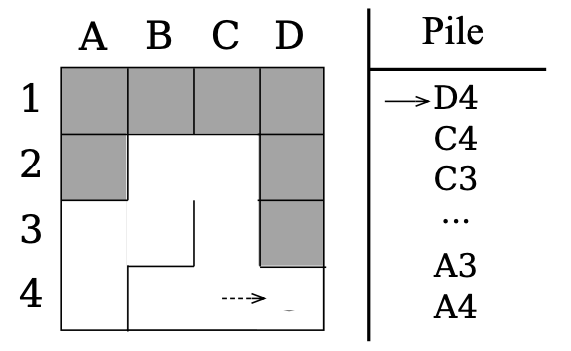
\includegraphics[width=\linewidth]{report/pics/backtracking6.png}
\end{minipage}

\begin{minipage}{0.6\textwidth}
Le processus se poursuit de cette manière, en revenant en arrière à chaque fois qu'on tombe sur une cellule ne possédant pas de voisins visitable jusqu'à ce que chaque cellule du labyrinthe ait été visitée.
\end{minipage}
\begin{minipage}{0.4\textwidth}
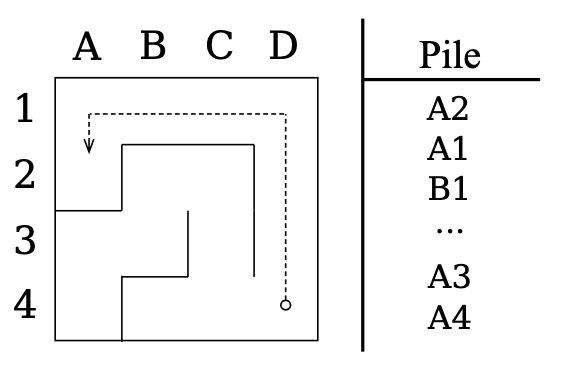
\includegraphics[width=\linewidth]{report/pics/backtracking7.png}
\end{minipage}


\begin{minipage}{0.6\textwidth}
La dernière cellule à visiter sera toujours une cellule n'ayant pas de voisins visitables. Nous revenons alors sur nos pas, en dépilant les cellules de la pile, à la recherche d'un voisin nos visité. Cependant dans notre cas, l'ensemble des cellules du labyrinthe ont été visitées, on dépilera alors les cellules jusqu'à revenir à notre cellule de départ (la cellule A4) qu'on supprimera également de la pile, ce qui nous laisse avec une pile vide.
\end{minipage}
\begin{minipage}{0.4\textwidth}
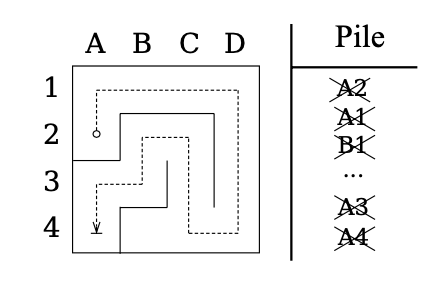
\includegraphics[width=\linewidth]{report/pics/backtracking9.png}
\end{minipage}

\begin{minipage}{0.6\textwidth}
Une pile vide est le signal de terminaison de l'algorithme. On se retrouve alors avec le résultat final qui est un labyrinthe parfait.
\\

\end{minipage}
\begin{minipage}{0.42\textwidth}
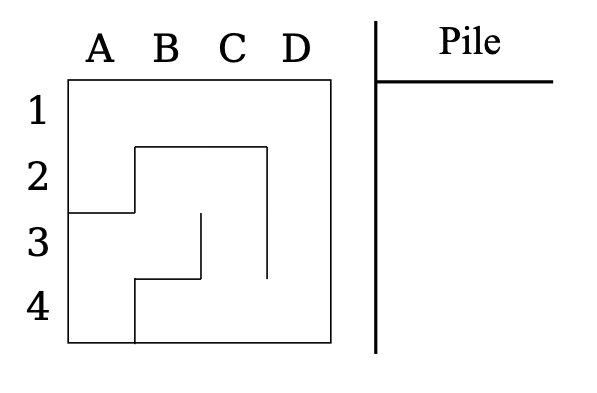
\includegraphics[width=\linewidth]{report/pics/backtracking8.png}
\end{minipage}

Sur les figures ci-dessous, on montre différents labyrinthes parfaits générés par notre algorithme de Backtracking une fois ce dernier implémenté.
\fig{pics/perfect1.png}{10.5cm}{11cm}
{Génération d'un labyrinthe parfait 8*8 dans notre simulation.}{mmcomp}
\newpage

\fig{pics/perfect2.png}{10.5cm}{11cm}
{Génération d'un labyrinthe parfait 12*12 dans notre simulation.}{mmcomp}

\fig{pics/perfect3.png}{10.5cm}{11cm}
{Génération d'un labyrinthe parfait 16*16 dans notre simulation.}{mmcomp}

\subsection{Génération de labyrinthes imparfaits}
Une des propriétées de base d'un labyrinthe parfait et qu'il existe un seul et unique chemin reliant deux cellules du labyrinthe. Cette propriété n'est pas respecté dans un labyrinthe imparfait, tel qu'il peut exister des boucles ou plusieurs chemins reliant deux cellules. Un labyrinthe imparfait peut être intéressant dans le cas ou l'on souhaite avoir plusieurs parcours possible entre deux cellules du labyrinthe afin de tester l'intelligence de notre Micromouse. Par exemple, dans le cas ou notre Micromouse démarre d'une cellule de départ A, qu'elle a pour objectif d'atteindre la cellule B, et qu'entre ces deux cellules il existe plus d'un chemin possible, on souhaiterais qu'après un certain nombre de parcours la Micromouse puisse distinguer entre les deux chemins et choisir le chemin optimal (le chemin le plus court).
\\
\newline
On génère un labyrinthe imparfait de la manière suivante :

\begin{enumerate}
    \item On commence d'abord par générer un labyrinthe parfait.
    \item Initialiser la position de la cellule départ (cellule sur laquelle démarre la Micromouse) et la cellule objectif (cellule que doit atteindre la Micromouse)
    \item On divise les cellules du labyrinthe en deux ensemble : l'ensemble "départ" et l'ensemble "objectif". La classification se fait sur le critère de proximité des cellules, les cellules les plus proches de la cellule départ seront mises dans l'ensemble départ et les cellules les plus proches de la cellule objectif seront mises dans l'ensemble objectif.
    \item Chercher un mur du labyrinthe qui sépare les deux régions (ensemble) et le supprimer.
    \\
    \newline
\end{enumerate}

On peut voir sur la figure ci-dessous le processus de génération d'un labyrinthe imparfait : 

\fig{pics/imperfect1.png}{7.5cm}{5cm}
{Génération d'un labyrinthe 6*6 imparfait.}{mmcomp}

Sur la figure ci-dessous est illustrée un labyrinthe imparfait généré par notre algorithme au sein de notre simulation : 
\newpage
\fig{pics/imperfect2.png}{10.5cm}{11cm}
{Génération d'un labyrinthe 8*8 imparfait dans notre simulation.}{mmcomp}

